\begin{surferIntroPage}{Kılavuz}{tutorial_koord1}{SURFER'da ilk adımlar}
Bu yazılımın adı SURFER. Okunduğunda muhtemelen aklınıza sörf/sörfçü sözcükleri geliyordur; yani su, güneş, dalgalar vs.  Oysa bu ad yabancı dillerdeki {\it surface} (yüzey) sözcüğünden geliyor.
\\
SURFER ile yüzeyleri, daha doğrusu cebirsel yüzeyleri resmedebilirsiniz. Bunun ne demek olduğu ve cebirsel yüzeylerin ne olduğu bu kılavuzda açıklanıyor. Kılavuzun bölümlerinde gezinmek için
sağ tarafta görülen yüzeylerden birini seçebilirsiniz.\\
SURFER yazılımı, 2008 Alman Matematik Yılı'nda başlayan gezgin IMAGINARY sergisinin bir parçası. Bu sergi Almanya'da Kara Ormanlar'da bulunan uluslararası üne sahip Oberwolfach
Matematiksel Araştırma Enstitüsü'nün (Mathematisches Forschungsinstitut Oberwolfach) bir projesi.
Enstitüde her hafta matematiksel araştırmalarda yeni konulara ilişkin çalıştaylar düzenleniyor.
Bu çalıştaylar, dünyanın her köşesinden bilim insanları arasındaki alışverişi desteklemek açısından çok önemliler. \\
\vspace{0.2cm} \hspace{3.5cm}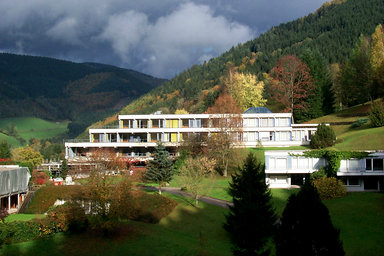
\includegraphics[width=3cm]{photo_mfo.jpg}\\
Açık ve özgür SURFER yazılımı internet sitemizden indirilebilir: \\
\begin{centering}
www.imaginary-exhibition.com\\
\end{centering}
 \vspace{0.2cm}
Sağınızda Limon yüzeyinden başlayarak matematiksel kılavuzları teker teker seçebilirsiniz.
Sol taraftaysa diğer galerilere atlayabilirsiniz, örneğin albenili yüzeylere...
\end{surferIntroPage}
